\ifdefined\included
\else
\setcounter{chapter}{3} %% Numéro du chapitre précédent ;)
\dominitoc
\faketableofcontents
\fi

\chapter{Elaborating a route for a human partner based on semantic knowledge}
\chaptermark{Elaborating a route for a human partner}
\label{chap:3}
\minitoc

In this chapter, we propose a representation of indoor environments in a semantic way by building a minimal but sufficient ontology, oriented around a route description task. This representation is then used to plan a route that a human has to follow to reach a goal destination. Finally, from the computed route a second process allows the robot to verbalize the route, seen as a procedure to be followed, allowing the guided human to mentally navigate along the route.

The contribution presented in this chapter is excerpted from our work, published in the proceedings of the Spatial Language Understanding (SpLU) 2019 workshop~\cite{sarthou_2019_semantic}. In this manuscript, the contribution is more detailed and discussed. This work is part of the \acrshort{mummer} project, aiming at developing a robot guide in a mall. At the end of this document (Chapter~\ref{chap:8}), a chapter is dedicated to the presentation of the project and the integration of the current contribution in a robotic system.

\section{Introduction}

We all have already been requested, or have ourselves asked for, for a route in a city, in a shopping center, or more simply in a house. When providing such information to a person, we perform what is commonly called a guidance task. Even if it can seem trivial for us, developing a robot able to perform it can be challenging. In this chapter, we choose to focus on the sub-task consisting at generating the explanation sentence. This sub-task is called the route description. To perform it, we first need a set of knowledge about the environment in which the guided person will walk, such as the paths, the intersections of the paths, or the elements alongside them. Then, we need a set of ``good practices'' to provide a route easy enough to follow and to remember.

In the \acrfull{hri} field, robots guides have been studied intensively and deployed into shopping centers~\cite{okuno_2009_providing}, museums~\cite{burgard_1999_museum, clodic_2006_rackham, siegwart_2003_robox}, or airport~\cite{triebel_2016_spencer}. From a knowledge representation point of view, we can notice the use of metrical representations~\cite{thrun_2007_simultaneous} or topological representations~\cite{morales_2011_modeling} to represent the environment in which the robot acts. Since we focus on the route description task, we consider that the robot does not accompany the human to his final destination but rather explains how to reach it. Consequently, the metrical representation will not be considered as being mainly used for navigation purpose~\cite{thrun_2007_simultaneous}. To perform more specifically a route description, topological knowledge is not sufficient. In addition to the topology of the environment, the robot needs to know the types of the elements composing the environment and their names in natural language. Some contributions have thus tried to mix metric or topologic representations with semantic ones to hold this additional knowledge~\cite {satake_2015_should, chrastil_2014_cognitive, zender_2008_conceptual}. However, mixing them can create a lack of uniformity among the overall knowledge representation. In this way, creating a unique representation allowing a robot to compute routes and expressing them could ensure uniformity among the knowledge.

Even equipped with a consistent representation of its environment, the robot has to find a route not for itself but for the guided human. A robot accompanying the human only has to determine a path, adapted to its capacities and interpretable only by itself. Providing a route to a human, the route has to be adapted to the human capabilities and knowledge. For example, in an outdoor environment, we will not give the same route for a car driver or a cyclist. In the context of a mall, we will not give a route with stairs to a mobility-impaired person or to someone with a shopping cart. Once computed, the robot has to explain the route. Where interactive maps only have to highlight a path, here, the robot has to generate a sentence that the human will be able to memorize. For sure the robot will not instruct a human with a sentence like ``walk 30 meters them turn -90 degrees''. This would not be adapted. The use of orientation and reference to elements of the environment will be needed through a sentence like ``walk until the florist then turn left''. We thus want the robot to generate plans understandable and executable by the human.

The first contribution of this chapter is a \textbf{unified representation} of an indoor environment using an ontology, to include both topological and semantic knowledge. Then, on the basis of this representation, we propose a first algorithm to \textbf{find a suitable route} to be explained to a human and a second algorithm to \textbf{verbalize a route} in an appropriate way.

%concerning semantic representation of indoor environment and
First, we review the literature on route description. Then, we introduce our unified semantic representation under the name of \acrfull{ssr}. We then present the algorithm used to compute the route and in a second time the algorithm to verbalize the previously computed route. We end this chapter with experimental results on both mockup and real environments.

\section[Related work]{Related work: the route description task}

%\subsection{Describing a route}

In the literature, a route description task is defined as being a particular kind of spatial description. First, from a cognitivist point of view, Denis in~\cite{denis_1997_description} has identified three main cognitive operations used to generate such a spatial discourse: 1) the activation of an internal representation of the environment, 2) the planning of a route in this representation, 3) and finally the formulation of the procedure to follow. From a computer science point of view, Cassell~\cite{cassell_2007_trading} considers the second operation as the fact of finding a set of route segments, each connecting two important points, and the third operation as chronologically explaining the route segments. In the same way, Mallot in~\cite{mallot_2009_embodied}, sees the second operation as the fact of selecting a sequence of places leading to the objective, and the third as managing declarative knowledge to choose the right action to be explained at each point of the sequence. While both second operations are equivalent, the third about the formulation of the procedure are rather complementary.

The route description task has been extensively studied in linguistic through verbal and textual communication to understand how humans communicate spatial knowledge. The goal of such studies has been to identify the invariants but also the good practices ensuring the success of the task. Through five experiments in both urban and indoor environments, Allen~\cite{allen_2000_principles} has identified three basic practices seen as being important for communicating knowledge about routes. They can be summarized as follows: a) respect the spatiotemporal order, b) concentrate on the information about the points of choice and c) use landmarks that the listener can easily identify.

This latter practice about the use of landmarks, also called reference marks, has been identified by Tversky~\cite{tversky_1999_pictorial} as a critical piece of information for the success of a route description. \cite{tversky_1998_space} finds that in addition to information about actions, reorientation, and direction, 91\% of the guidance instructions contains the use of landmarks. These results confirm the ones of~\cite{denis_1997_description}. Montello~\cite{montello_1993_scale} tries to identify when the use of landmarks appears in a description. Defining the \textit{Vista} space as being the area within sight and the \textit{Environmental} as being the rest of the environment reachable through locomotion, he finds that guides usually use landmarks when the target places are no longer in the \textit{Vista} space but in the \textit{Environmental} one. Moreover, with regard to~\cite{tversky_1999_pictorial}, the use of landmarks appears during an explanation of a direction changing. In addition, their choice is based on salient features over a route description~\cite{nothegger_2004_selection}.

\begin{figure}[ht!]
\centering
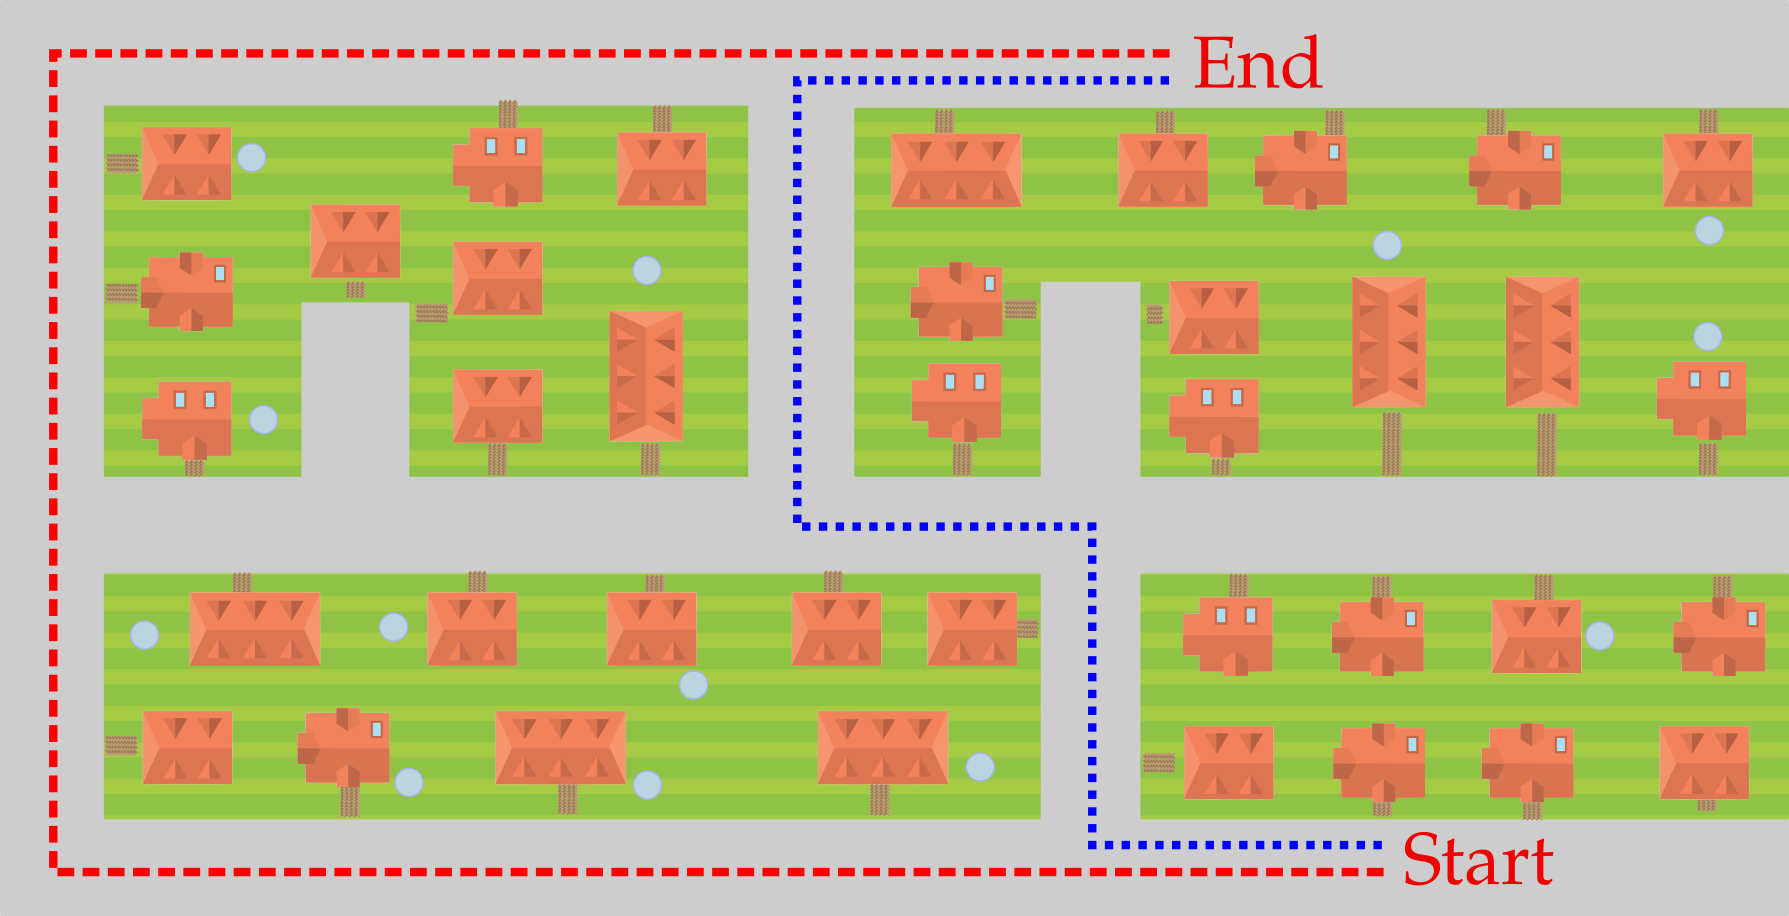
\includegraphics[scale=0.22]{figures/chapter3/landscape/landscape.png}
\caption{\label{fig:chap3_shortest} Comparison of two routes in terms of complexity and length. Even if the blue route (. . .) is the shortest, many directions changing are required. Each of them is a risk for the guided person to make a mistake and be lost again. The red route (- - -), although being a bit longer, is easier to explain and to remember, and has few directions changing.}
\end{figure}

Even if the use of landmarks helps at understanding direction changing by anchoring in the environment the action to be performed, there is still a risk for the guided person to make a mistake, taking the wrong path. While the length of the route is an important criterion in the choice of a route, its complexity has also to be taken into account when we need to explain it. Morales~\cite{morales_2015_building} argued that reducing the route complexity, in terms of the number of stages composing it, should be preferred to its length. This feature reduces the risk of mistakes concerning the choice to make along the route and also has an impact on its understanding and memorization. This criteria of minimal explanation can be compared to the Grice's Maxim of quality~\cite{grice_1975_logic}. In the example of Figure~\ref{fig:chap3_shortest}, some should prefer to explain the red route rather than the blue one, even if it is longer, since it is easier to remember.

Finally, to explain the same route, Taylor~\cite{taylor_1992_spatial} has noticed that a speaker can use two kinds of perspectives. First, the \textit{survey} perspective tend to adopt a bird's eye view point of the environment, meaning a top view of it like looking at a map. With this perspective, the speaker refers to the different landmarks of the route with respect to one another. They are thus referred to using terms including north-south-east-west. This perspective is opposite to the \textit{route} perspective. With such a perspective, the speaker mentally navigates along the route, making an imaginary tour of the environment. As a result, he refers to the landmarks with respect to the future guided person position along the route. The landmarks are thus referred to using terms like left, right, front, or back. \cite{taylor_1996_perspective} notices that the survey perspective is generally used for open environments whereas the route perspective is generally used in environments with already identified paths. For indoor environments, the route perspective should thus be preferred to facilitate route understanding and memorization.

%\subsection{Environment represention to compute routes}

%Regarding the environment representation generally used to find itineraries, we can first take a look at GNSS road navigation systems. In \cite{liu_1997_route} or \cite{cao_2009_gps}, we find the same principle of a topological network representing the roads with semantic information attached to each of them. Such representation seems adapted regarding the performance required for such systems operating in very large areas. However, GNSS road navigation systems must respond only to this unique task of finding a route where a robot is expected to be able to answer various tasks and unprecise destination requests. For our application, we thus need a representation that can be used more widely while still allowing the search for routes.

%Satake in~\cite{satake_2015_field} has developed a topological graph for the route search process. To understand the human request about the destination node in the graph, they build an ontology, providing a semantic description of them. The description informs about the places types (e.g. cloth shop, restaurant, ...), names and nicknames, and the sold items. However, as explained in~\cite{morales_2015_building}, such a map with annotated elements does not provide a suitable base to generate route explanations using a route perspective. Nevertheless, we can note that the use of an ontology, if suitable to describe the meaning of the elements of the environment. In the same way, you can also describe other elements than shops, like stairs, elevators, entrances, or escalators. To unify the representations, we could thus, represent the topology in an ontology. Since both are graphs, this representation should be feasible and provide more information about the elements along the paths.

%To semantically represent an environment, Kuipers in~\cite{kuipers_2000_spatial} introduce the Spatial Semantic Hierarchy (SSH). With it, he defines a 'topological level' composed of three main elements being the places, paths, and regions, as well as relations between them. To create our semantic description of an indoor environment, we thus choose to take it as a basis. The concepts definition will be refined in the next section.

%Since this contribution is focused on a pattern to describe environment and algorithms using it the compute routes, the presented representation are made by hand. However, many contributions trend to automatically generate a topological graphs from geometric measurements (e.g. Region Adjacency Graphs \cite{kuipers_2004_local}, Cell and Portal Graphs \cite{lefebvre_2003_automatic}, hierarchical models \cite{lorenz_2006_hybrid}, or from natural language \cite{hemachandra_2014_learning}). Even if we do not have used such techniques for the moment, our contribution could benefit from these works, solving the complexity of creating such a representation by hand.

\section{The Semantic Spatial Representation}

Satake~\cite{satake_2015_field} has developed a topological graph for the route search process. To understand the human request about the destination node in the graph, they build an ontology, providing a semantic description of them. The description informs about the places types (e.g. cloth shop, restaurant, ...), names and nicknames, and the sold items. However, as explained in~\cite{morales_2015_building}, such a map with annotated elements does not provide a suitable base to generate route explanations using a route perspective as it misses directional information. Nevertheless, we can note that the use of an ontology is suitable to describe the meaning of the elements of the environment. In the same way, one can also describe other elements than shops, like stairs, elevators, entrances, or escalators. To unify the representations, we could thus, represent the topology in an ontology. Since both are graphs, this representation should be feasible and provide more information about the elements along the paths. As explained in the previous chapters of this thesis, ontologies are widely used for knowledge representation, to capture the meaning of the elements of an environment but also to encode knowledge dedicated to the robot's internal process. In this way, they provide a good interface between the robot's processes and its human partner in terms of interaction.% Where Satake~\cite{satake_2015_field} already use an ontology to describe the different shops of a shopping center, in this section, a present how to represent the topology of the environment in addition.

To semantically represent an environment, Kuipers in~\cite{kuipers_2000_spatial} introduces the Spatial Semantic Hierarchy (SSH). He defines a 'topological level' composed of three main elements being the places, paths, and regions, as well as relations between them. To create our semantic description of an indoor environment, we thus choose to take it as a basis. However, this representation does not use an ontology, we thus present how we extend it to represent the topology in an ontology. The resulting representation and its underline pattern are what we will call the \acrfull{ssr}.

Since this contribution is focused on a pattern to describe environments and algorithms using it to compute routes, the presented representations are made by hand. However, many contributions trend to automatically generate a topological graph from geometric measurements (e.g. Region Adjacency Graphs \cite{kuipers_2004_local}, Cell and Portal Graphs \cite{lefebvre_2003_automatic}, hierarchical models \cite{lorenz_2006_hybrid}, or from natural language \cite{hemachandra_2014_learning}). Even if we do not have used such techniques for the moment, our contribution could benefit from these works, solving the complexity of creating such a representation by hand.

In the following, we first present the used classes and properties before ending with an example of a description.

\subsection{The SSR classes}

Kuipers has defined three distinct concepts being the \textbf{region}, the \textbf{path}, and the \textbf{place}. To represent the topology, we have refined the concepts of place and path. Here below, we define these concepts and their refinement. The resulting class hierarchy is representing with the TBox of Figure~\ref{fig:chap3_tbox}.

\begin{figure}[ht!]
\centering
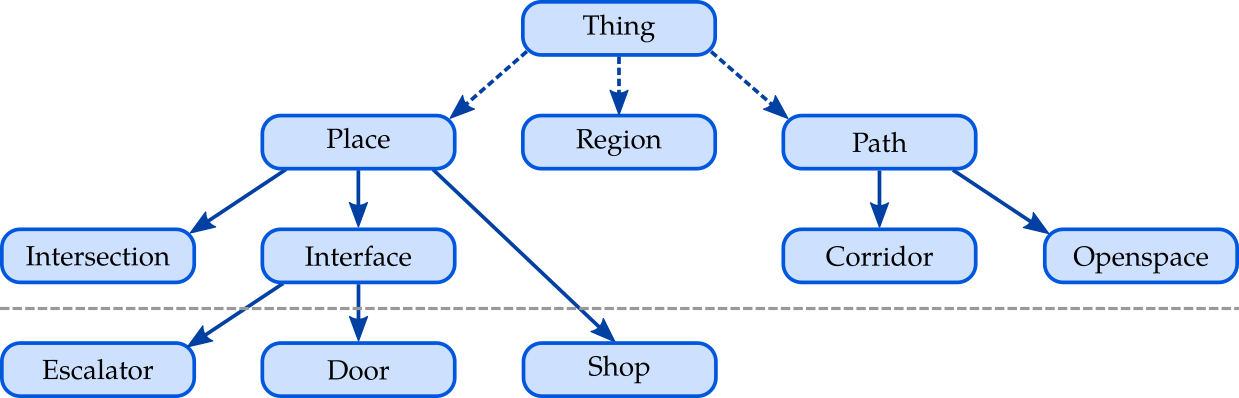
\includegraphics[scale=0.4]{figures/chapter3/ssr_tbox.png}
\caption{\label{fig:chap3_tbox} Representation of the TBox (classes hierarchy) of the \acrlong{ssr} used to describe the topology of an indoor environment. While the top part is inherent to the \acrshort{ssr}, the bottom one extends the latter to provide more granularity.}
\end{figure}

\paragraph{Region:} It represents a two-dimensional element, drawing an area. An area is a subset of an overall environment. A description of an environment must include at least one region being the entire environment itself. However, defining multiple regions aims at creating a finer representation. For example, for multi-storey buildings, we will at least represent each floor by a distinct region. Regions can be described as being nested if needed.

\paragraph{Path:} It is a one-dimensional element, like a line. We can materialize it as an element along which it is possible to move by following it. Even if it is not directly semantically represented, a path must have a direction in order to describe other elements in relation to it. A path can be refined into:

\begin{itemize}
  \item \textbf{Corridor:} It represents a kind of path having a distinct beginning and end. In this way, a corridor cannot be a loop. The direction of the corridor can be chosen arbitrarily. However, its direction defines the position of its beginning and end. Consequently, it also defines the right and left of the corridor. The direction does not mean that the corridor can be used in a unique way but will be used to describe the elements along with it.
  \item \textbf{Open space:} It is a kind of path which does not have any defined beginning or end. It thus forms a loop. It can also be viewed as a ``potato-shaped'' describing the outline of open space. It materializes the possibility of turning the gaze around the room and the fact of not having to go through a defined path to reach one of its points. In a building, a hall would typically be described with such a path.
\end{itemize}

\paragraph{Place:} It represents a point of zero dimension\footnote{For sure it has a 3D location, but here we are speaking of its use in navigation from one place to another.}. It can either represent a physical or symbolic element. In the context of a mall description, a shop would inherit the place class as a point representing its door can be sufficient to describe it. To represent the topology, we refine it into:
  
\begin{itemize}
  \item \textbf{Path intersection:} It represents the connection between two and only two paths. It is thus a waypoint to go from one path to another. In the case of a crossing between three paths, three intersections have to be described.
  \item \textbf{Interface:} It represents the connection between two and only two regions. It is thus a waypoint to move from one region to another. It can be physical, like a door or a staircase, or symbolic like a passage.
\end{itemize}

To better catch the difference between paths and places, it can be related to the differences between the types of rooms made by~\cite{andresen_2016_wayfinding}. Some rooms in a building such as a house have the main use to circulate from a room to another, they are corridors. Other rooms have an explicit use that is not the traffic, they are places even if you can move in.

\subsection{The SSR properties}

The relations introduced by Kuipers aim at representing the connections of places and paths, the order of the places along a path, and the elements in the regions. The main relations are the following:

\begin{align*}
&on(place,path) && place \text{ is on } path \\
&order(path,place1,place2,dir) && \text{the order on } path \text{ from } place1 \text{ to } place2 \text{ is } dir \\
&right\_of(path,dir,region) && path \text{, facing direction } dir \text{, has } region \text{on its right}\\
&left\_of(path,dir,region) && path \text{, facing direction } dir \text{, has } region \text{on its left} \\
&in(place,region) && place \text{ is in } region
\end{align*}

Through these relations, we can first see a slight difference in our use of the main elements. The regions are used to group a set of places along a path, avoiding in this way to describe each individual place as being at the right/left of a path. That way, our use of the concept of region will thus require more description for each place but has the advantage to give a finer granularity of huge environments representation with a first level of abstraction. With it, we could imagine a short prior description like ``it is on the first floor''.

A major limitation of these relations is that they cannot be used in an ontology as they are not all in the form of triplets. The issue comes from the need for a direction to determine the order and the side positions. The properties we introduce aim at fixing this issue and give a more precise description. For example, with the representation of Kuipers, we cannot have a place at the edge of a path. All the properties presented here can be extended with their inverse (e.g. $isIn$ and $hasIn$) for a more expressive model and thus easier handling. The resulting property hierarchy is represented with the partial RBox of Figure~\ref{fig:chap3_rbox} 

\begin{figure}[ht!]
\centering
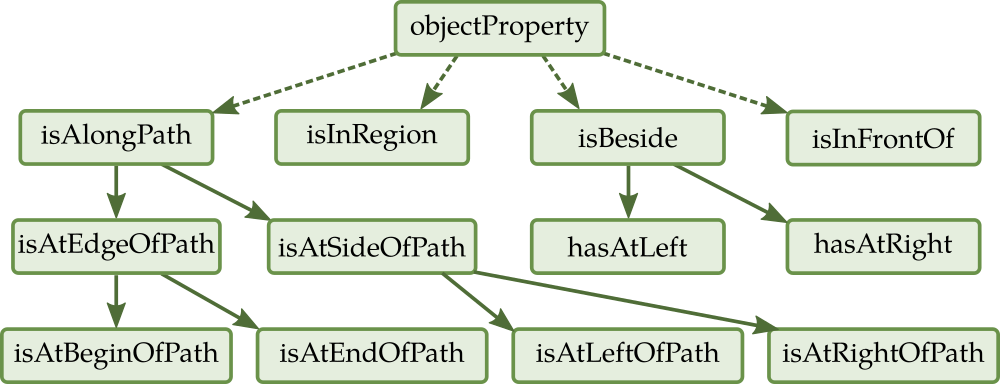
\includegraphics[scale=0.42]{figures/chapter3/ssr_rbox.png}
\caption{\label{fig:chap3_rbox} Representation fo the RBox (properties hierarchy) of the \acrlong{ssr} used to describe the topology of an indoor environment.}
\end{figure}

\paragraph{isInRegion:} $isInRegion(path/place,\ region)$ describes the fact that a $path$ or a $place$ is in a $region$.

\paragraph{isAlongPath:} $isAlongPath(place,\ path)$ describes the fact that a $place$ is along $path$. Depending if the path is a corridor or an openspace, a finer description can be needed:
\begin{itemize}
  
  \item $isAlong(place,\ corridor)$: Since a corridor is a line, the places along the path can first be described as being either on a side of the corridor with the property $isAtSideOfPath$ or at the edge with the property $isAtEdgeOfPath$. Thanks to direction of the corridor, these properties can be refined with $isAtBeginOfPath$ and $isAtEndOfPath$ for the places at an edge, and  $isAtRightOfPath$ and $isAtLeftOfPath$ for the places along a side of the corridor. Even if the direction of the corridor is not directly represented in the ontology, since the places have been positioned in relation to the direction, we can retrieve it.
  \item $isAlong(place,\ openspace)$: For open spaces, since they do not have a beginning or an end, places are only defined as being along with an open space.
\end{itemize}

\paragraph{isBeside:} $isBeside(place1,place2)$ describes the fact that $place1$ is beside $place2$. To really represent their order, we use the properties $hasAtLeft$ and $hasAtRight$. The choice of these properties is made by positioning themselves at the place and facing the path the place is along.

\paragraph{isInfrontOf:} $isInfrontOf(place1,place2)$ describes the fact that $place1$ is in front of $place2$. This property is not mandatory for all the places but provides a finer description. The more it is used, the more the verbalization of the itinerary will be easy. We will see in the sentence generation section that it is however important to always define a place in front of an intersection. This information will be used to determine if the guided human will have to go left or right in some cases. If there is no described place in front of an intersection, we can use a $emptyPlace$ class that would inherit the $place$ class.

To simplify the description few axioms are made. The property $isInfrontOf$ is defined as reflexive. The properties $hasAtRight$ and $hasAtLeft$ are defined as inverse from one another. Finally the chain axiom $isAlong \bullet isIn \rightarrow isIn$ is used to not have to set the $isIn$ property for each place. It can be deduced thanks to the path they are along.

\subsection{An example of description}

To illustrate the use of our \acrshort{ssr}, we will describe the shop $pl\_5$ (with the red floor) represented in Figure~\ref{fig:chap3_example}. For the description of this place, we will use the previously introduced classes and properties.

\begin{figure}[ht!]
\centering
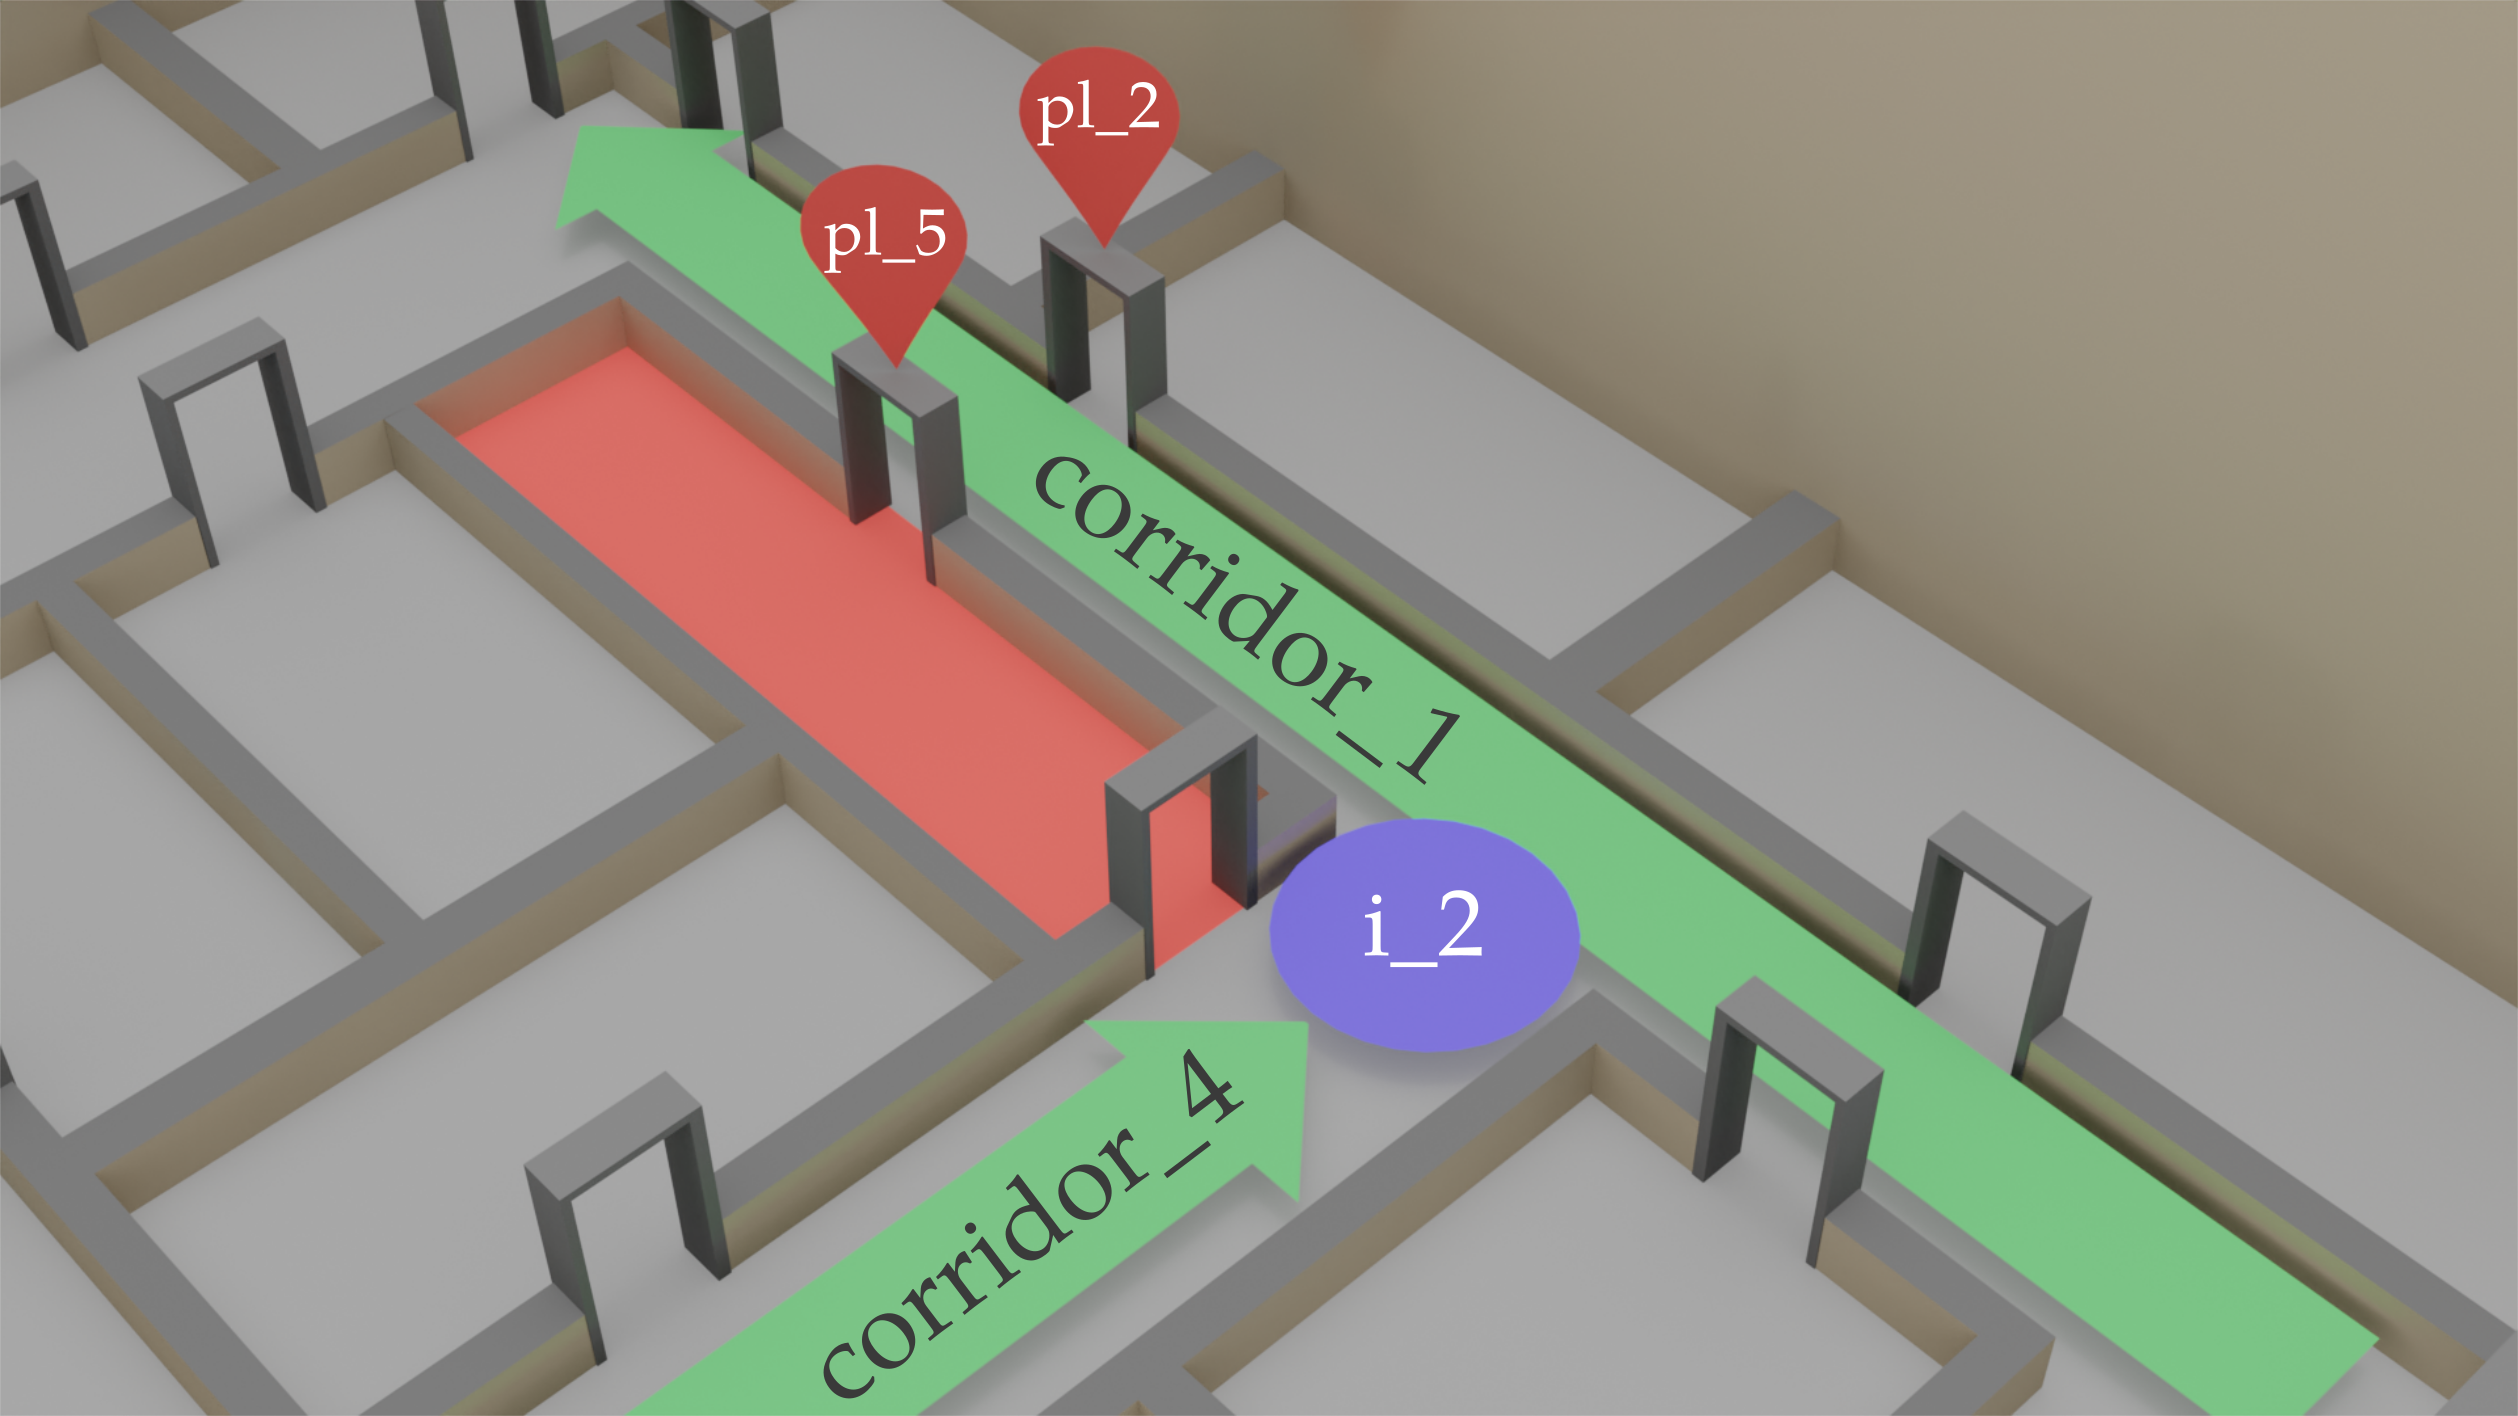
\includegraphics[scale=0.16]{figures/chapter3/SSR_example.png}
\caption{\label{fig:chap3_example} An example of environment with two corridors, an intersection, and two shops represented as places. All the elements are in the same region. The arrows represent the corridors directions.}
\end{figure}

To describe our environment, we start with the description of its paths. The corresponding ontology is available in Listing~\ref{lst:chap3_corridors}. In the example, we have two corridors. We assume that both are in a common region named $region\_1$. The paths do not need further description. To pass from one to the other, we create an intersection, here denoted $i\_2$. To describe its position along with the two paths we have to take a look at the paths' directions. For $corridor\_4$, the intersection is at its end edge. For $corridor\_1$, the intersection is at its left.

\begin{lstlisting}[frame=single, basicstyle=\scriptsize\ttfamily, label={lst:chap3_corridors}, caption={Description of the two corridors and their common intersection in the OWL language using the Turle syntax.},captionpos=b, style=OwlTurtle_indiv]
:corridor_1  rdf:type     :Corridor ;
             :isInRegion  :region_1 .
             
:corridor_4  rdf:type     :Corridor ;
             :isInRegion  :region_1 .
             
:i_2  rdf:type        :Intersection ;
      :isAtEndOfPath  :corridor_4;
      :isAtLeftOfPath :corridor_1.
\end{lstlisting}

Once the paths and intersections are described, we can describe the other places of the environment. For this example, we only describe the shop $pl\_5$. We would do the same process for all the others. The place $pl\_5$ is first a shop,  which is a particular kind of place. Regarding the corridors, it is at the left of $corridor\_1$. However, it also has an entrance overlooking $corridor\_4$. We can thus describe it as being along two paths. Depending on the starting point of the description, we will be able to instruct for one of its two entrances. For $corridor\_4$, $pl\_5$ is at its left. Now that the place is positioned along paths, we have to describe its position according to its adjacent places. Facing $corridor\_1$, the intersection $i\_2$ is at the right of $pl\_5$ and the shop $pl\_2$ is in front of it. Facing $corridor\_4$, the intersection would be at its left. However, $pl\_5$ is on a side of the corridor while $i\_2$ is at one of its edges. Consequently, we do not have to describe any order between them. The resulting ontology part is provided in Listing~\ref{lst:chap3_pl5}.

\begin{lstlisting}[frame=single, basicstyle=\scriptsize\ttfamily, label={lst:chap3_pl5}, caption={Description of the shop pl\_5 using the \acrshort{ssr} in the OWL language using the Turle syntax.},captionpos=b, style=OwlTurtle_indiv]
:pl_5  rdf:type         :Shop ;
       :isAtLeftOfPath  :corridor_4 ;
       :isAtLeftOfPath  :corridor_1 ;
       :hasAtRight      :i_2 ;
       :isInFrontOf     :pl_2.
\end{lstlisting}

\section{Finding routes: A two-level search}

At this point, we have created and built a representation of the environment using the \acrfull{ssr}. Using this representation, we now want to compute routes from one place to another. We already saw that even if the length of a route can be a criterion, the complexity of the description is a more important criterion when we have to describe it. Moreover, depending on the guided person, some routes could be prefered to others, to avoid stairs, to favor elevators, or to reduce the use of potentially crowded paths.

In this section, the goal is to provide multiple routes so that we can then choose the best route based on personal preferences, during the interaction. In order to reduce the complexity of this exhaustive search, especially for large scale environments, we propose to work at two levels:
\begin{itemize}
\item \textbf{First} the region-level. It considers only regions and interfaces such as doors, stairs, or elevators. In such a way, we will not consider paths in regions not leading to the goal destination. If we are on the ground floor and want to go to a place also on the ground floor, exploring other floors would be useless.
\item \textbf{Then} the place-level. It provides complete routes computation including paths and intersections within regions.
\end{itemize}

\subsection{The region-level: Trim down the search}

\begin{figure}[b!]
\centering
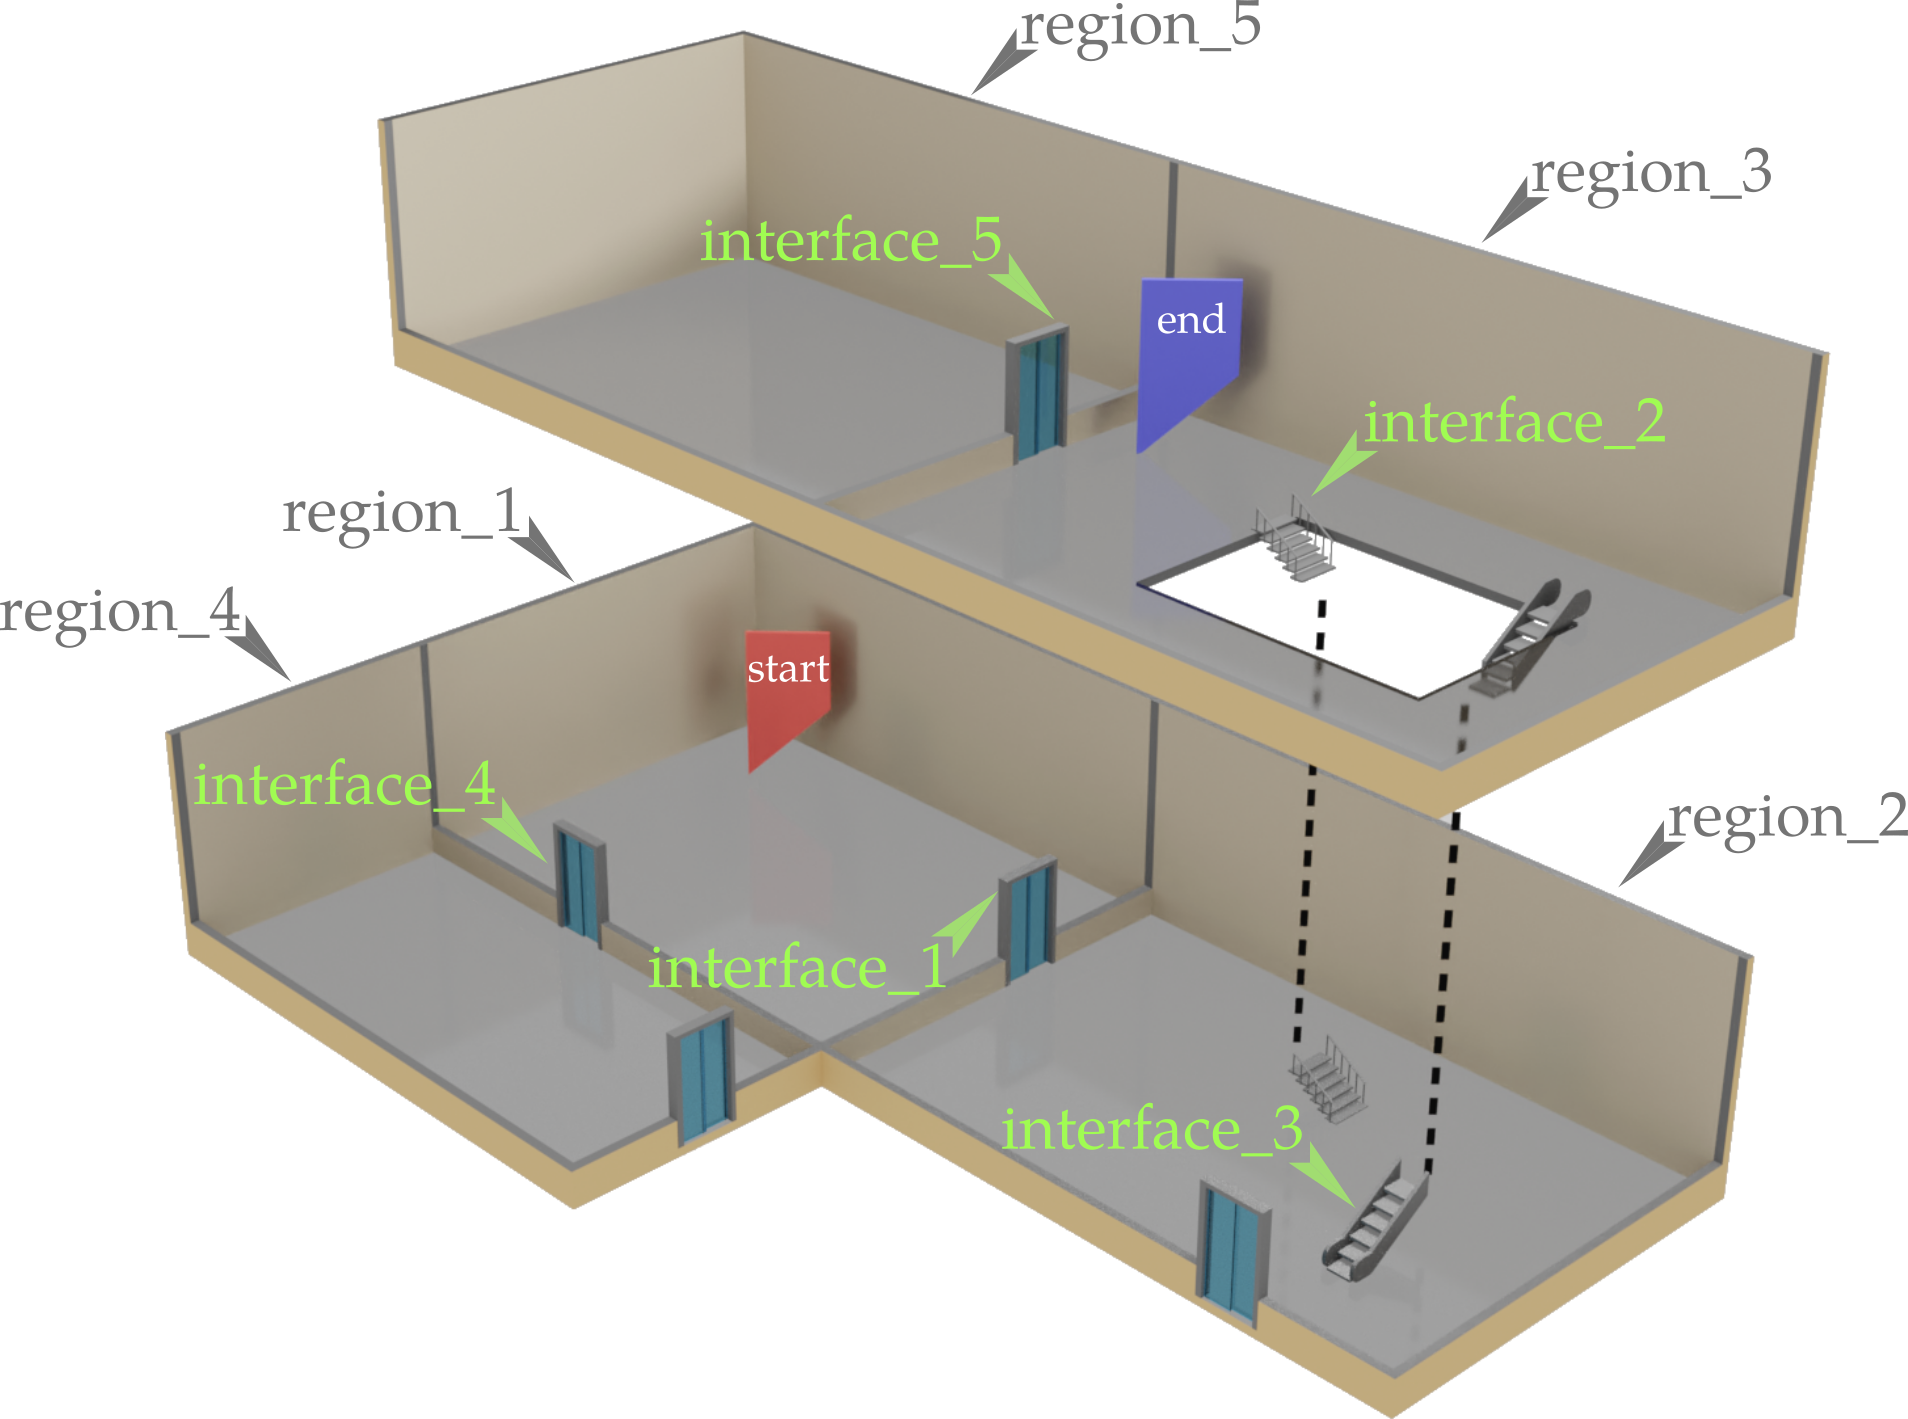
\includegraphics[scale=0.22]{figures/chapter3/building_regions.png}
\caption{\label{fig:chap3_regions} Representation of an environment at the region-level. Regions are linked through interfaces. We know that the starting point of the search is in \textit{region\_1} and the goal place is in \textit{region\_3}. }
\end{figure}

In large-scale environments such as multi-storey buildings, routes computation can lead to combinatorial explosion. Exploration at the region-level can decrease this effect, giving a first high-level exploration. To study this first level, we take the example of Figure~\ref{fig:chap3_regions}. It represents a building composed of five regions. Each is linked to others through the use of interfaces, being doors, stairs, or escalators. In this environment, the goal is to guide a human from the flag ``start'' to the flag ``end''. Quickly analysing this figure, we can see that the human will have to pass by regions 1, 2, and 3. To pass from \textit{region\_1} to \textit{region\_2} the only interface is \textit{interface\_1}. To pass from \textit{region\_2} to \textit{region\_3}, two interfaces can be used, either \textit{interface\_2} or \textit{interface\_3}. The exploration of the two other regions is useless.

For this first level of exploration, we only use the regions and the interfaces as they link the regions. Since the places are along paths and the paths are in regions, we know in which region is each place. Using the property \textit{isInRegion}, we get the starting region and the goal region respectively from the start place and the end place. In our example, we get that the human has to go from \textit{region\_1} to \textit{region\_3}. These two regions define the initial state and goal state of a search algorithm. Considering the regions as the nodes of a graph and the interfaces as its edges, we can thus apply a graph search algorithm to find routes at the region-level.

\begin{algorithm}[!htb]
\caption{Exhaustive Graph Search algorithm for region exploration}
\label{alg:chap3_region_search}
\begin{algorithmic}[1]
\Function{Exhaustive\_region\_search}{$problem$}
	\State $state \leftarrow$ ($problem$.initial\_region, \_) 
    \State $frontier\leftarrow$ a FIFO queue of state
    \State $frontier\leftarrow$ \textsc{INSERT}($state$, $frontier$)
    \State $solutions\leftarrow$ an empty set
    \\
    \Loop
        \If{\textsc{empty}($frontier$)} 
        	\State \Return $solutions$
        \EndIf
        \\
        \State $state\leftarrow$ \textsc{pop}($frontier$)
        \If{$state$.current\_region is $problem$.goal\_region } 
        	\State $solutions\leftarrow$ \textsc{INSERT}($state$, $solutions$)
        \Else
        	\ForAll{$interface$ of $state$.current\_region.hasInRegion s.t. $\notin state$}
        		\ForAll{$region$ s.t. $interface$.isInRegion}
        			\If{$region \notin state$} 
        				\State $frontier\leftarrow$ \textsc{INSERT}($state \cup$ ($region$, $interface$), $frontier$)
        			\EndIf
        		\EndFor
        	\EndFor
        \EndIf
    \EndLoop
\EndFunction
\end{algorithmic}
\end{algorithm}

Since we want to provide several routes, we use the exhaustive graph search algorithm represented in Algorithm~\ref{alg:chap3_region_search}. Such an exhaustive search allows us to take into account all possible interfaces. In this algorithm, we consider a state as being a list of pairs composed of a region and the intersection used to come to the region. The initial state (line 2) thus takes the initial region and no interface. When we explore a state (line 11) we first test if its current region (the last one in the list) is the goal region (line 12). If it is, rather than returning the state, we simply add it to a solution set (line 13). If the current region is not the goal one, we retrieve from the ontology all the interfaces connected to the current region thanks to the property \textit{hasInRegion} which is the inverse of \textit{isInRegion}. For each of these interfaces not already used in the state (line 15), we get the regions it is connected to (line 16). With each of these regions not already used in the state (line 17), we finally create a new state which is added to the frontier (line 18). The algorithm only stops when no more state has to be explored (line 8). By including the knowledge base exploration directly inside the search algorithms, it is not necessary to extract a topological graph with nodes and edges. It is carried out within the search algorithm without preprocessing.

\begin{figure}[ht!]
\centering
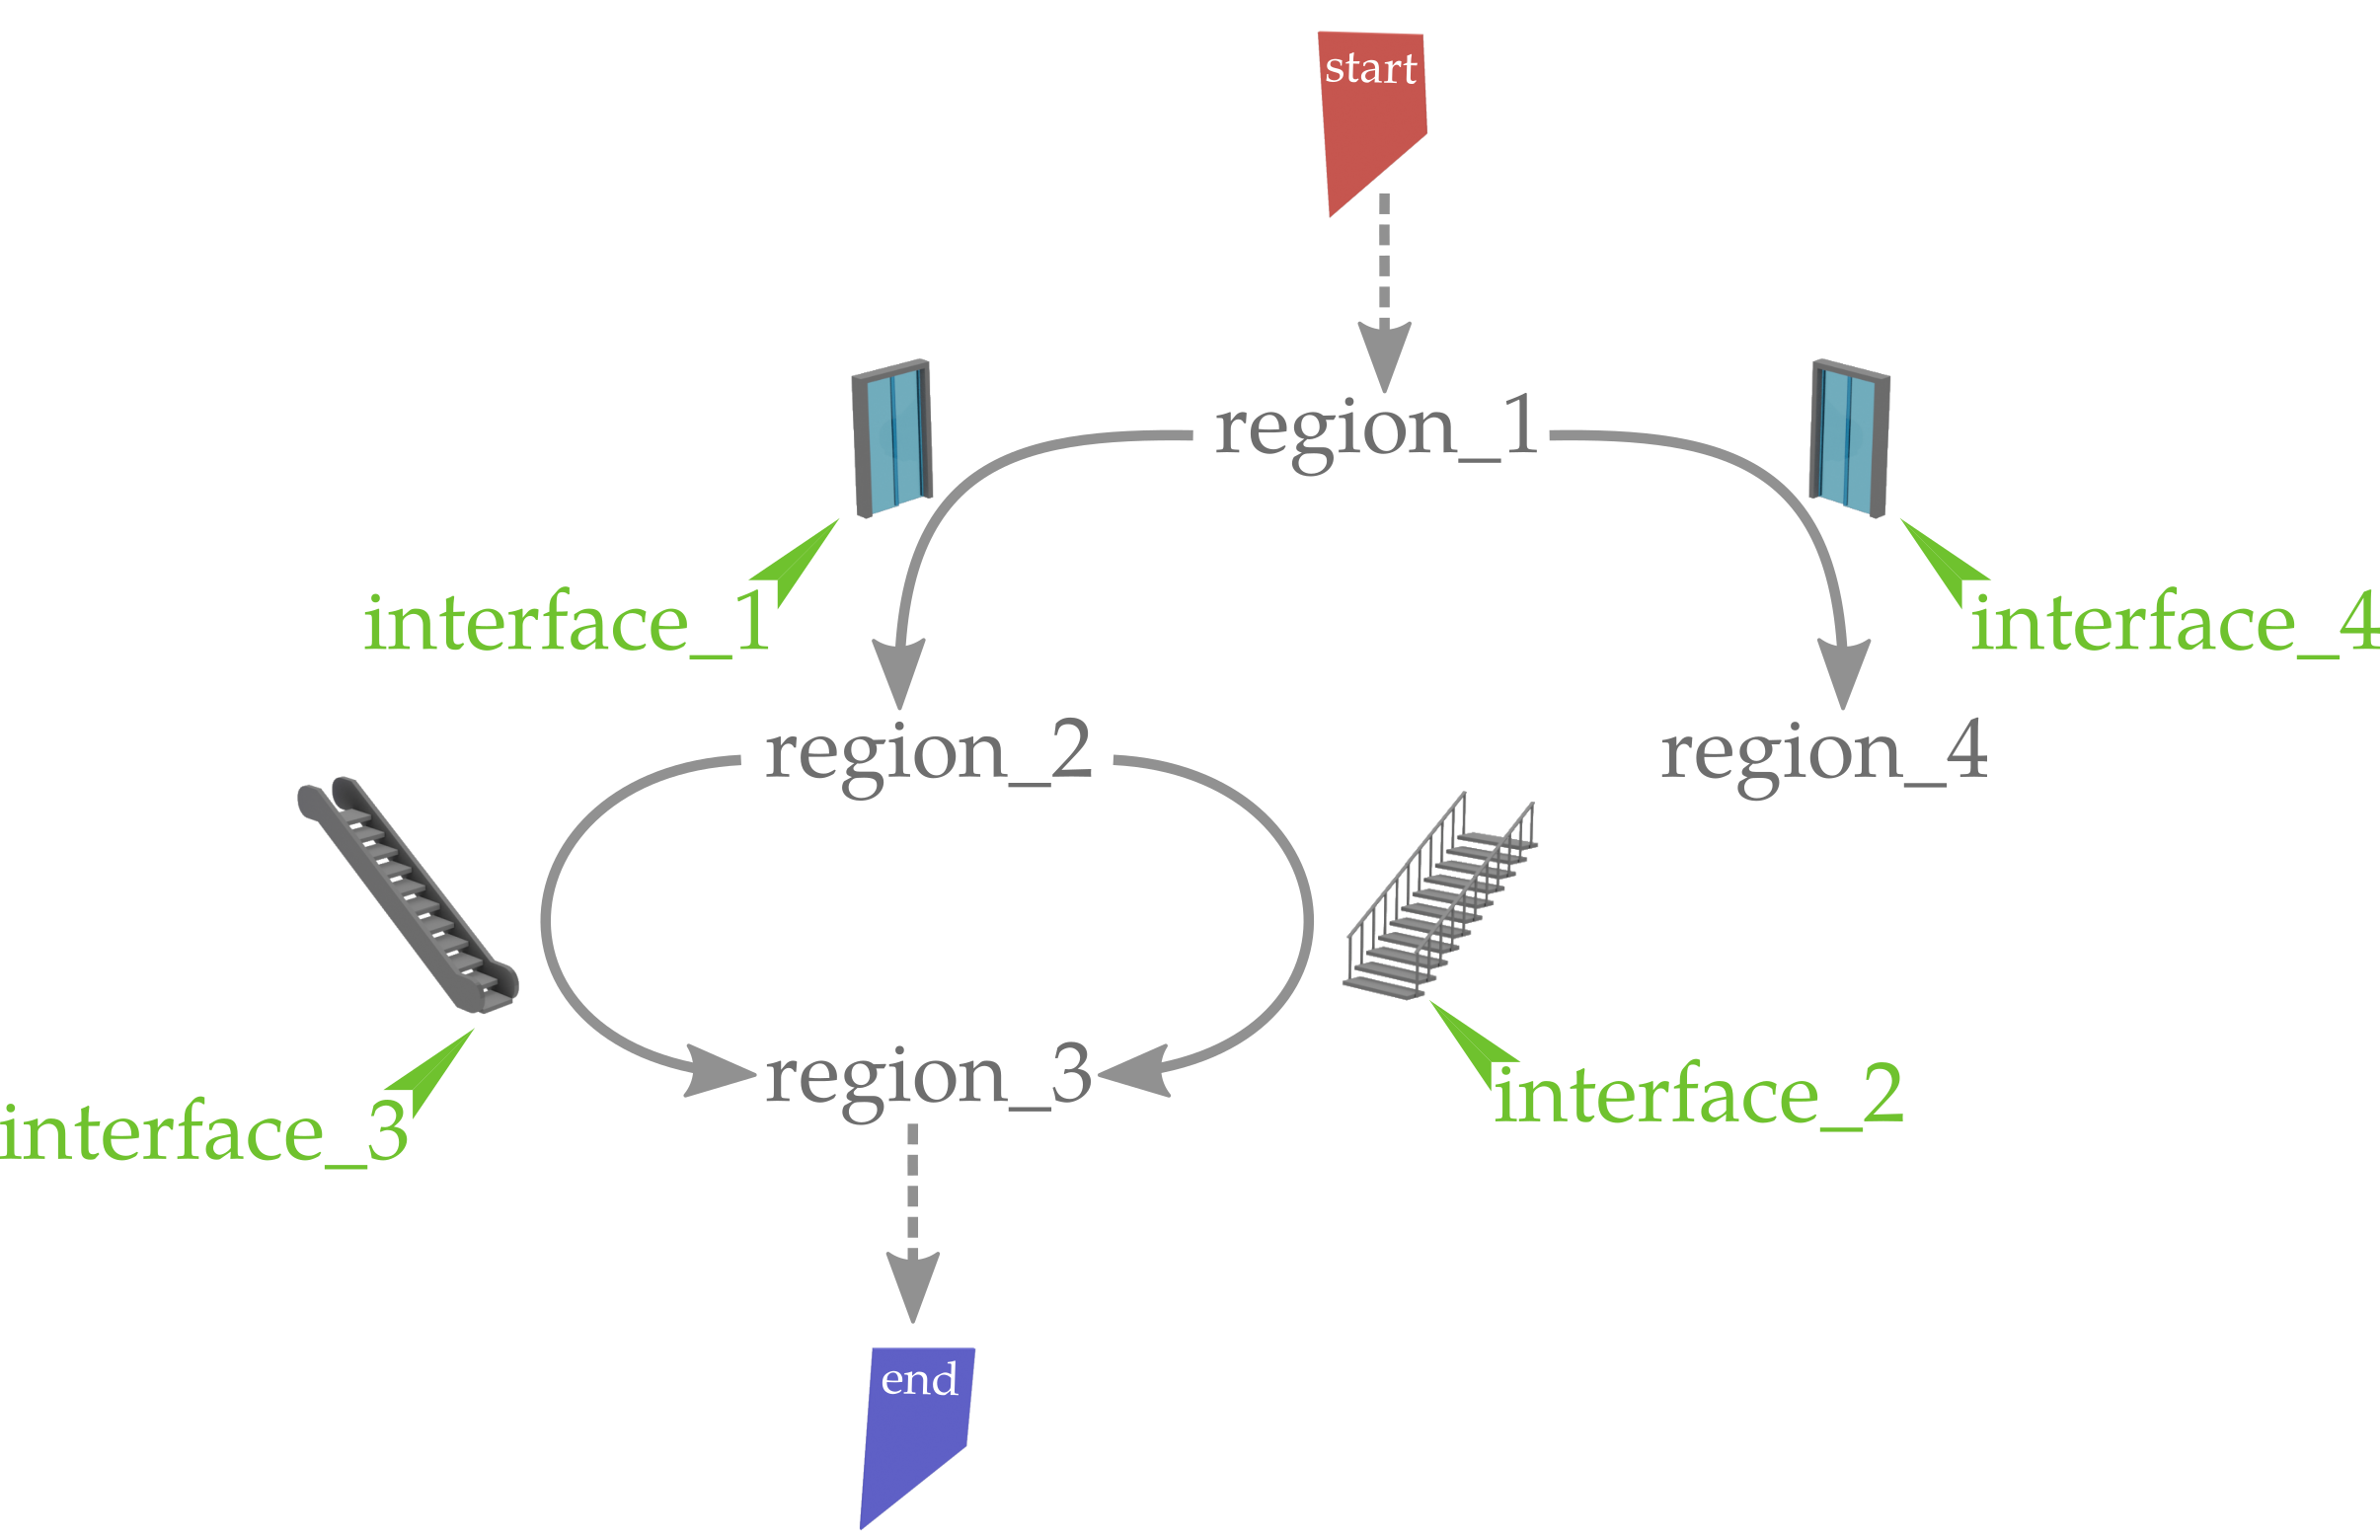
\includegraphics[scale=0.12]{figures/chapter3/Region_exploration_graph.png}
\caption{\label{fig:chap3_region_expl} An illustartion of the exploration process at the region-level for the example of Figure~\ref{fig:chap3_regions}.}
\end{figure}

The exploration performed by this algorithm on our example is illustrated in Figure~\ref{fig:chap3_region_expl}. The \textit{region\_4} has been detected as being a deadend and the \textit{region\_5} has not been explored at all. The two found solutions are the routes:

\begin{align*}
region\_1 - interface\_1 - region\_2 - interface\_2 - region\_3 \\
region\_1 - interface\_1 - region\_2 - interface\_3 - region\_3
\end{align*}

This type of result makes it possible to quickly eliminate unnecessary regions to be analysed next and thus reduces the complexity for a more detailed search at a second time. This technique is similar to what is done for GNSS road navigation systems where the main roads are studied upstream of secondary roads with pyramidal (or hierarchical) route structure \cite{bovy_2012_route}.

\subsection{The place-level: Refine the search}

Place-level search is based on the Region-level search results with the aggregation of start and end places. The format changes from:
\begin{gather*}
region - place - region - ... - region \\
\text{to} \\
\textbf{place} - region - place - region - ... - region - \textbf{place}
\end{gather*}

Place-level search works from one place to another through a single region. We have therefore divided the previous solutions to meet this constraint. This step aims to reduce complexity again. Indeed, several routes can pass through the same region with the same places of departure and arrival. The inner route can thus be calculated once and for all. In our example, the division gives five sub-routes instead of six:

\begin{align*}
&start - region\_1 - interface\_1 \\
&interface\_1 - region\_2 - interface\_2 \\
&interface\_2 - region\_3 - end \\
&interface\_1 - region\_2 - interface\_3 \\
&interface\_3 - region\_3 - end
\end{align*}

The place-level algorithm aims to replace each region in the sub-routes with a succession of paths and intersections. Focusing on \textit{region\_1}, illustrated in Figure~\ref{fig:chap3_region1}, we need to find a route from the start place to \textit{intersection\_1}. Using the property \textit{isAlongPath}, we get from the ontology that the starting place is along \textit{corridor\_1} and the interface 1 (\textit{i\_1}) is along \textit{corridor\_5}. Solving it by hand, a possible solution would be to take \textit{corridor\_1}, then pass by the intersection 1 (\textit{i\_1}) to reach \textit{corridor\_5}.

\begin{figure}[ht!]
\centering
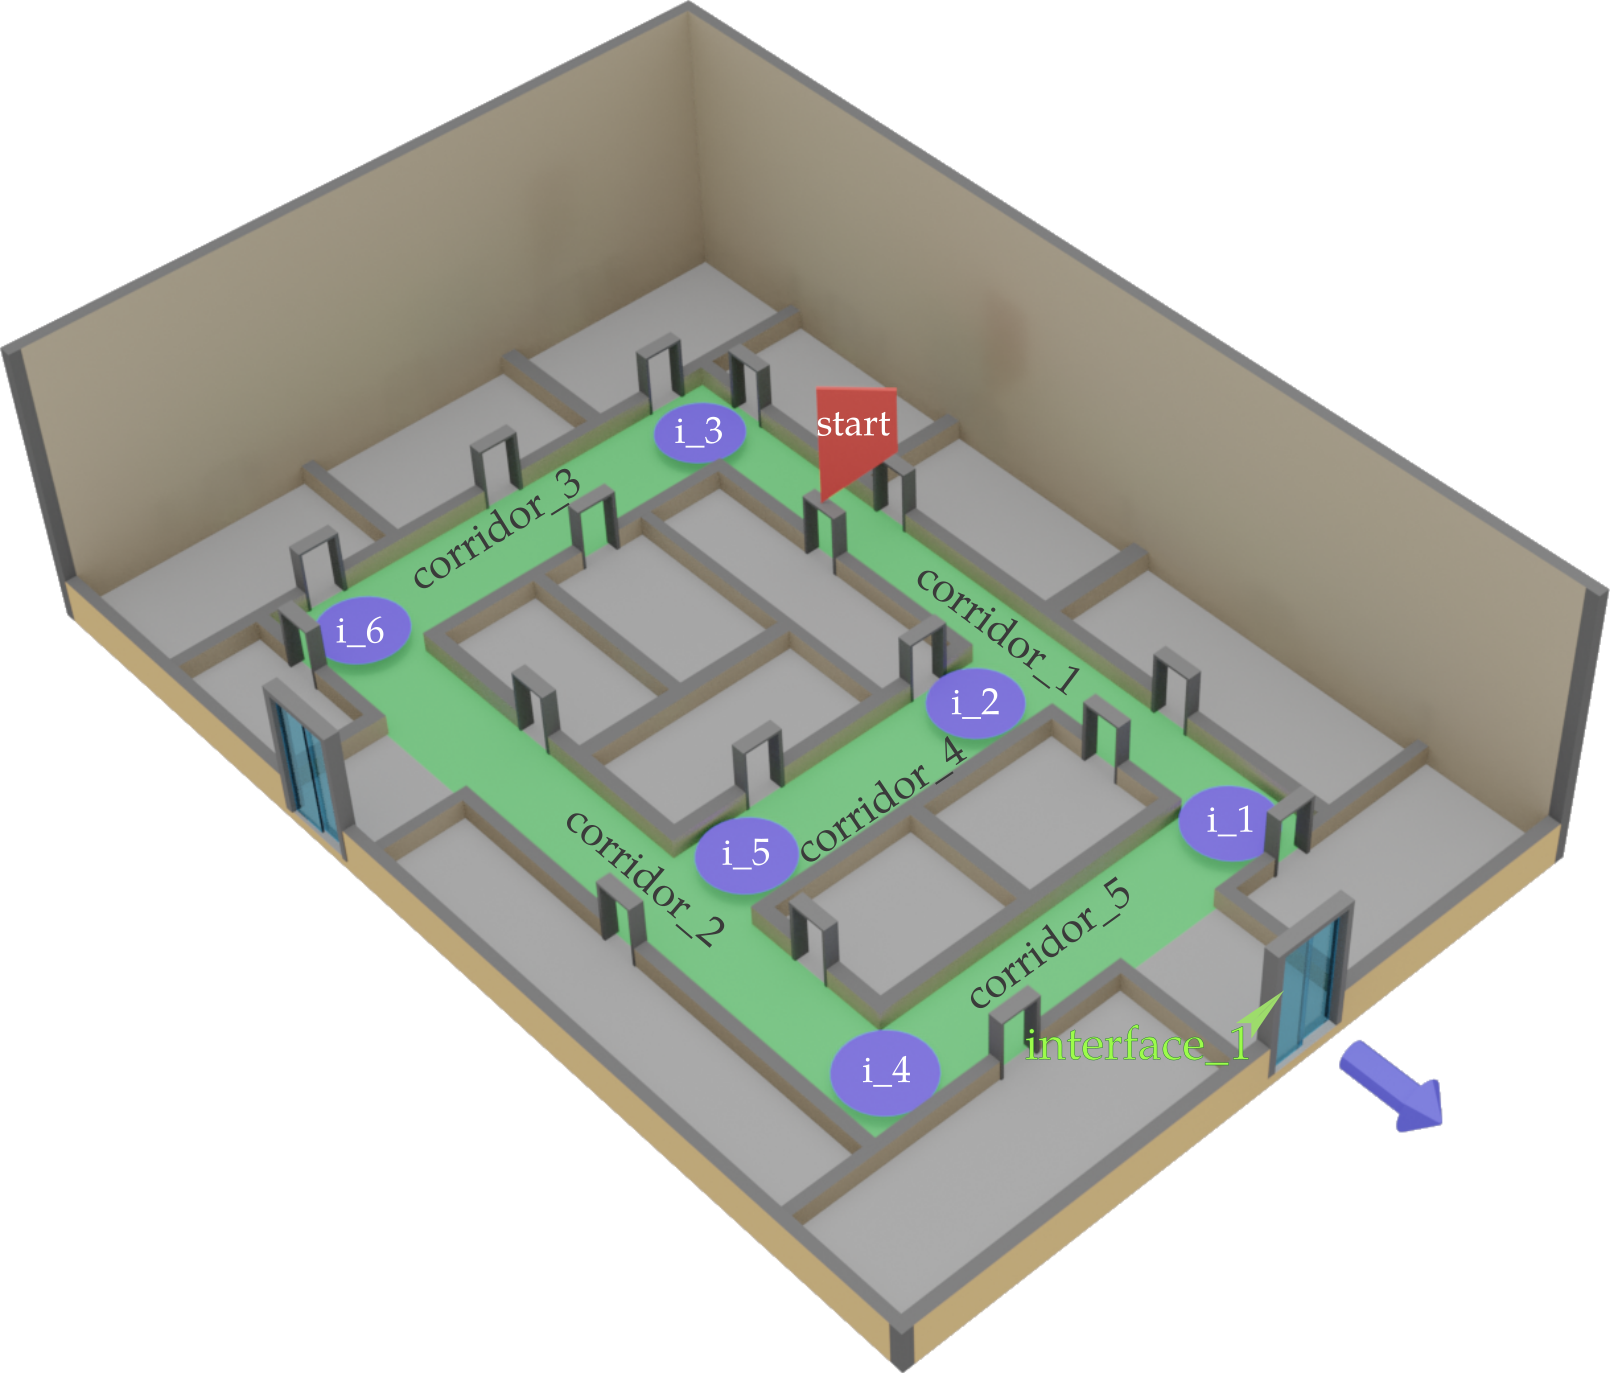
\includegraphics[scale=0.28]{figures/chapter3/region1.png}
\caption{\label{fig:chap3_region1} Representation of \textit{region\_1} at the place-level. A region is composed of paths (here corridors only) connected through intersections. We know that the starting point of the search is along \textit{corridor\_1} and the local goal place is in \textit{corridor\_5}. }
\end{figure}

Whereas at the region-level an exhaustive search was acceptable due to the limited number of regions and their limited connectivity, such a search cannot be applied to the place-level. In our example of \textit{region\_1} we could find four routes, without loops, to go from the start place to \textit{interface\_1}. In a more realistic environment, it could be of the order of several tens. We thus choose to only get the less complex route, at the place-level, for each sub-route. Since the complexity of the route is only impacted by the number of items composing the route, a not cost-based algorithm can be used. Moreover, considering the places of the region as nodes and the paths as edges, we thus have a graph. To find the optimal route in a graph without costs associated with the edges or nodes, we choose a breadth-first algorithm. Its pseudocode is provided in Algorithm~\ref{alg:chap3_path_search}.

\begin{algorithm}[ht!]
\caption{Adapted breadth-first search algorithm for paths exploration. This version does not return the first valid solution but all the solutions having the same minimum length.}
\label{alg:chap3_path_search}
\begin{algorithmic}[1]
\Function{Exhaustive\_path\_search}{$problem$}
    \State $frontier\leftarrow$ a FIFO queue of state
    \State $explored\leftarrow$ a set of explored path
    \State $solutions\leftarrow$ an empty set
    \State $min\_length \leftarrow inf$ 
    \\
    \ForAll{$path \in problem$.initial\_paths}
    	\State $state \leftarrow$ ($path$, \_) 
    	\State $explored\leftarrow$ \textsc{INSERT}($path$, $explored$)
    	\If{$path \notin problem$.goal\_paths}
    		\State \Return $state$
    	\Else
    		\State $frontier\leftarrow$ \textsc{INSERT}($state$, $frontier$)
    	\EndIf
    \EndFor
    \\
    \Loop
        \If{\textsc{empty}($frontier$)} 
        	\State \Return $solutions$
        \EndIf
        \\
        \State $state\leftarrow$ \textsc{pop}($frontier$)
        \ForAll{$intersection$ s.t. $state$.current\_path.hasAlong $\land \notin state$}
        	\ForAll{$path$ s.t. $intersection$.isAlong $\land \notin state$}
        		\If{$path \in problem$.goal\_paths}
        			\State $state \leftarrow state \cup$ ($path$, $intersection$)
        			\If{$state$.size $\leq min\_length$}
        				\State $solutions\leftarrow$ \textsc{INSERT}($state$), $solutions$)
        				\State $min\_length \leftarrow state$.size
        			\EndIf
        		\ElsIf{$path \notin explored$}
        			\State $frontier\leftarrow$ \textsc{INSERT}($state \cup$ ($path$, $intersection$), $frontier$)
        			\State $explored\leftarrow$ \textsc{INSERT}($path$, $explored$)
        		\EndIf
        	\EndFor
        \EndFor
    \EndLoop
\EndFunction
\end{algorithmic}
\end{algorithm}

This algorithm has been adapted to better fit our problem. First of all, a place can be along several paths. In the case of our starting place, in addition to be along \textit{corridor\_1}, we have described it as being also along \textit{corridor\_4}. Performing a search for each combination of departure path and destination path would be time-consuming. Where a breadth-first algorithm commonly takes one initial state and one goal state, we have adapted it to assume several initial and goal states. This modification is visible from line 7 to line 12 of our algorithm. For each initial path, we create an initial state and test if it is one of the goal paths or not. We also put them all in the explored set to avoid to search route passing by them since we are already along with them. The second adaptation comes from the number of solutions. A breadth-first search only returns the shortest solution. However, if several solutions exist with the same length, only the first found is selected. Since we want to propose several routes, we do not exit the algorithm once a solution is found but rather bound it from there with the variable \textit{min\_length}. At line 23, any state having a size bigger than the minimum length is forsaken. Once all the routes under exploration reach this limit the frontier becomes empty and the algorithm stops.

This algorithm is applied to each sub-route found at the previous stage. The overall routes are then recomposed with the results found at the place-level. The final routes are in the form of:

\begin{gather*}
start\ place - path - place - ... - place - path - goal\ place
\end{gather*}

\section{Generating an explanation in natural language}

This section describes the third cognitive operation of \cite{denis_1997_description} to generate a spatial discourse: the formulation of the procedure. Similarly to \cite{cassell_2007_trading}, we define a route description as a set of route segments, each connecting two important points. Taking the format of the previously found routes, the segments correspond to each path of the route and the two places linked to. The segments have then to be verbalized in a chronological way. To generate the full explanation, we start with the determination of the actions to be performed and the computation of the positions of the landmarks along the route, taking the route perspective. Then, with this information, we present how we elaborate an explanation in natural language.

\subsection{Reconstructing the paths}

In the same way as \cite{tversky_1999_pictorial}, we consider that to enable their explanation, each segment of a route corresponds to a triplet: orientation, action, and landmark. A route description can thus be realized through the repetition of three steps: designating a landmark, reorienting the listener, and continuing the progression by prescribing an action.

The issue with the environment representation used to compute the route is that it is not directly usable to generate the formulation of the procedure. With the current representation, the orientation and action are too complex to extract, given that they depend on the direction by which the guided human arrives. Nevertheless, thanks to the additional information provided by the \acrlong{ssr}, it is possible to interpret the representation in relation to the estimated future position of the human. This interpretation is what we call an internal representation. It is an interpretation of the \acrshort{ssr} based on the current task. To generate the triplets of the segments, we create such an internal representation for each segment of the route to explain. The segments are thus represented and analysed independently from one another.

For the corridors, we start by defining four sets. These sets are used to represent the places at the left of a path, the places at its right, the places at its beginning, and the places at its end. Given the corridor \textit{c\_i} such that $(c\_i, Corridor) \in \inheritset$, the set of places $Pi_{right}$ at its right is:

\begin{gather*}
Pi_{right} = \{ pl\_i\ |\ (pl\_i,\ isAtRightOfPath,\ c\_i) \in \relationset \}
\end{gather*}

\begin{figure}[h!]
\centering
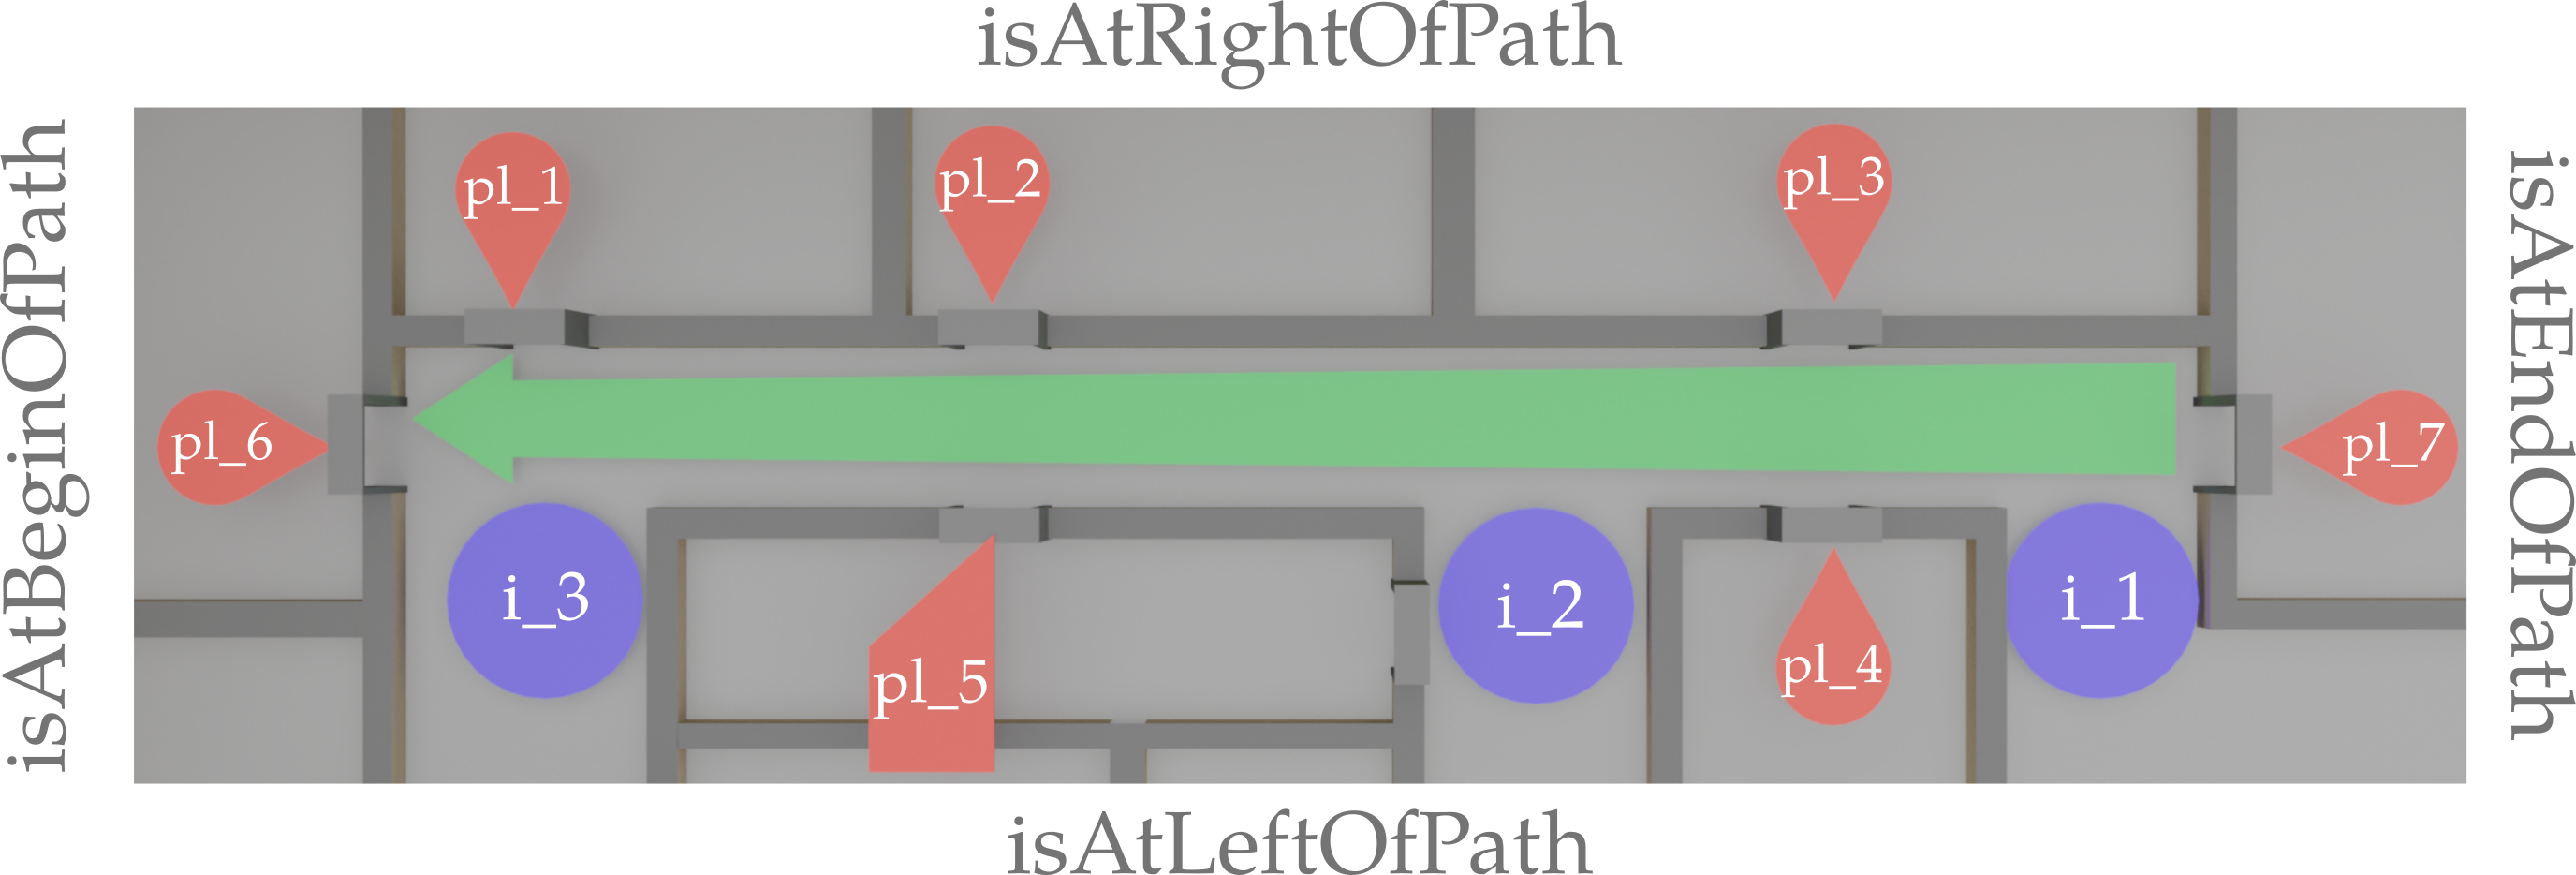
\includegraphics[width=\textwidth]{figures/chapter3/corridor.png}
\caption{\label{fig:chap3_corridor} Internal representation of a \textit{corridor\_1} extracted from the semantic representation. Thanks to the specialisations of the \textit{isAlongPath} property (i.e. \textit{isAtLeftOfPath}, ...) we know on which side of the path each place is. With the specialisations of the \textit{isBeside} property, we can reconstruct the order of the places for each side. }
\end{figure}

The three other sets are built in the way using relations including the properties $isAtLeftOfPath$, $isAtBeginOfPath$, and $isAtEndOfPath$. We then consider these sets as being partialy ordered sets (posets) through the binary relation~$<$. For two elements $a$ and $b$ of a set $Pi$, we said that $a\ <\ b$ if $(a,\ hasAtRight,\ b) \in \relationset$. Thanks to these four partially ordered sets\footnote{The sets are not totally ordered because we do not consider the transitivity of the relations $hasAtRight$ and $hasAtLeft$ directly in the ontology. Consequently not all the elements can be compared.} we can reconstruct the arrangement of a corridor like in Figure~\ref{fig:chap3_corridor} for \textit{corridor\_1} of our running example and of Figure~\ref{fig:chap3_pallokatu} for an automaticaly generated visualisation of the reconstruction of a corridor of a real mall (used in Chapter~\ref{chap:8}). To match the positions of places on opposite sides, we use the relations involving the property $isInFrontOf$.

\begin{figure}[ht!]
\centering
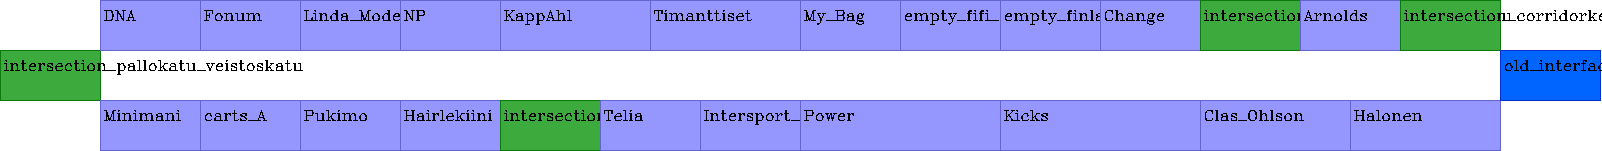
\includegraphics[width=\textwidth]{figures/chapter3/pallokatu.png}
\caption{\label{fig:chap3_pallokatu} An example of an automaticaly generated visualisation of a reconstruction based on the semantic knowledges. The places in green are intersections, the place in blue is an interface, and the others are shops. }
\end{figure}

For the open spaces, we only generate one partially ordered set representing all the locations along with it. We still use the property $isInFrontOf$ to improve the placement of the places.

\subsection{The robot putting itself in your shoes}

Once we have an internal representation of each segment, we can determine the procedure that the user must perform. Cassell in \cite{cassell_2007_trading} mentions that an action, a reorientation, a progression, or a positioning must be carried out at the end of each segment. The end of one segment being the beginning of the next, we choose to determine the actions at the beginning of each segment (which corresponds more precisely to our internal representation). It allows to work on one path at a time. This rule is formalized in \cite{mallot_2009_embodied} as:

\begin{gather*}
``choosing\ action\ A_i\ at\ place\ P_j\ will\ lead\ to\ place\ P_k''
\end{gather*}

This determination of actions can be made thanks to our internal representation. It is represented in red on the top of Figure~\ref{fig:chap3_directions} assuming the human to come from the place $pl\_5$ ($P_j$) and $P_k$ as being one of the other places of the corridor. For example, if the local place to reach is $pl\_1$ the action will be \textit{``turn left''}. If the local place to reach is $pl\_2$ the action will be \textit{``go in front of you''}. If the place is on the same side, the ordering of the set is sufficient to determine the action. If the place is on an edge, the action depends on the side from which the humans come and the edge to reach. If the place to reach is on the other side of the path, we have to use the property $isInFrontOf$ to determine the action to perform.

\begin{figure}[ht!]
\centering
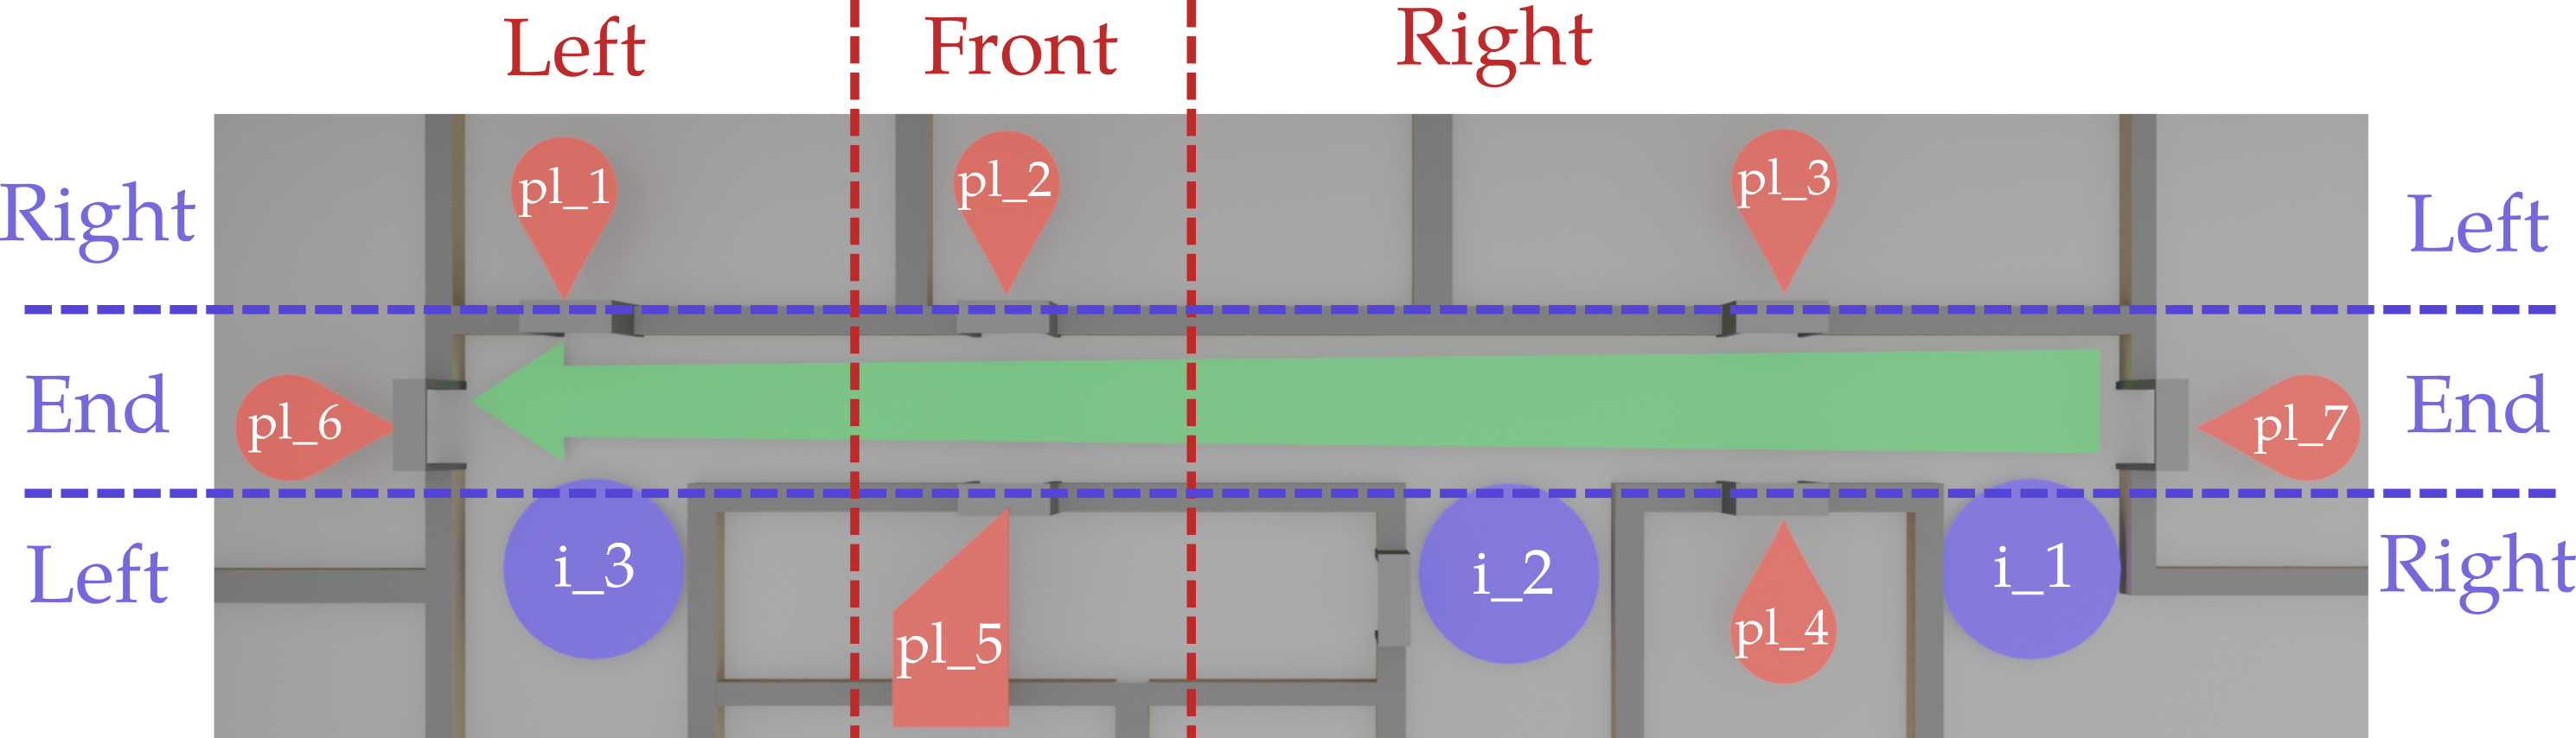
\includegraphics[width=\textwidth]{figures/chapter3/directions.png}
\caption{\label{fig:chap3_directions} In red (on top) is represented the resolution of the action to be performed (i.e. going in front, turning left, or turning right) from the starting place \textit{pl\_5}. In blue (on the sides) is represented the resolution of the position of the place to reach depending on the performed action. Starting from place \textit{pl\_5}, to reach the intersection \textit{i\_1}, the guided human will have to turn right (red) then the place will be on his right (blue). Starting from place \textit{pl\_5}, to reach the place \textit{pl\_3}, the guided human will have to turn left (red) then the place will be on his right (blue). }
\end{figure}

The information in blue on the two sides of Figure~\ref{fig:chap3_directions} gives the orientation of the sub-goal place $P_{k}$ taking into account the previous reorientation. With this orientation information, we can inform the guided human about the location of the next step once the previous action has been performed. Wanting to reach intersection $i\_1$, we can give the explanation \textit{``take the corridor at your right''}. The full sentence would thus be \textit{turn right then take the corridor on your right"}\footnote{We can note that this sentence can also lead to \textit{i\_2}. We will fix it after.}. Consequently, taking into account the orientation of the guided person after an action, we provide directions in the route perspective. The guided human can thus perform an imaginary tour of the environment~\cite{cassell_2007_trading}.

Working segment by segment in the order given by the route search algorithm, we necessarily generate the explanations with a spatiotemporal ordering. This criterion is an important point in Allen's best practice in communicating route knowledge \cite{allen_2000_principles}.

The latest critical information is the landmarks. With our internal representation, we provide all the landmarks (corresponding to places along the paths) around which action must be taken. In the previous example, the sentence may be confusing because there will have two corridors on the right. We are able to refer to place $pl\_4$ to ground the action. With this new information, a sentence without ambiguity would be \textit{``turn right then take the corridor at your right straight after pl\_4''}. With this last sentence, we can no longer go to \textit{i\_2}.

\subsection{A pattern-based generation}

In order to generate the sentences in natural language, we first analyzed explanations used by human guides in a human-human study \cite{belhassein_2017_human}. From this study, we have identified four types of explanation components: those corresponding to the beginning of the route, the end of the route, the progress in it, and the particular case of routes with only one step. Each type has sub-types of explanation components. For example, for the sentences expressing progress in the route, we can mention two sub-types: sentences expressing a redirection action and the ones expressing the fact of continuing forward. Thus, each explanation belongs to a sub-type according to the kind of information it expresses. This classification allows us to have multiple ways to express the same information, varying the robot turn of phrase and vocabulary when talking to a person. To represent similar sentences and to be able to generate sentences with variations, we have grouped sentences with close lexical structures. Each sentence is then represented with its variations through the use of patterns. An example of pattern is: [``you will''], [``see'', ``find''],[``it'', ``/X''], [``on''], [``your'', ``the''], [``/D''],[``side'',``when you walk'', ``'']. When using a sentence, the variations are randomly chosen with a uniform distribution. We can notice in the previous example the use of place-holders such as X or D. The place-holder X corresponds to the name of an element of the environment and D to a direction (right or left). We also implemented the use of a Y variable to refer to another element of the environment (a landmark) and DY to refer to its location. The pattern \textit{``You will see X at the DY of Y''}  becomes for example \textit{``You will see Burger King at the right of Espresso House''} after instantiation. If a sentence requires a variable that the algorithm is not able to extract from our internal representation, then we select another sentence with the same meaning or another variation of the sentence that does not require the previously used variable.

In our English verbalization, we have 238 unique patterns to express the end of a route description, 64 to express its beginning, 20 to express the continuation, and 66 for the special case of a route with a single step. All the patterns are available in appendix~\ref{app:patterns}.

For the example of Figure~\ref{fig:chap3_region1}, a possible verbalization would be:

\begin{quote} 
\centering 
\textit{
``Go through this corridor, turn right straight after pl\_4, then you will see the door on your left.''}
\end{quote}

For the same route, the system would be able to generate another sentence like:

\begin{quote} 
\centering 
\textit{
``Walk across this corridor and turn right straight after pl\_4. After that, the door is on the left there, straight after pl\_7.''}
\end{quote}

\section{Experiment in the mockup and the real environment}

The \acrshort{ssr} was first used to describe a mockup mall to test the related algorithms. This representation has then been tested in a real mall to study its applicability in a larger environment. Table~\ref{tab:chap3_count} indicates the number of elements described in both environments. The number of places does not correspond to the sum of the shops, interfaces and intersections since much more elements have been described, such as ATMs, restrooms or carts location. These two environments are detailed in Chapter~\ref{chap:8}.

\begin{table}[!ht]
\begin{center}
   \begin{tabular}{ | c || c | c | }
     \hline
                        & Mockup mall & Real mall \\ \hline \hline
     Places             & 83            & 251   \\ \hline
     Shops              & 19            & 140   \\ \hline
     Interfaces         & 11            & 18    \\ \hline
     Path intersections & 10            & 50    \\ \hline
     Paths              & 11            & 41    \\ \hline
     Regions            & 5             & 3     \\
     \hline
   \end{tabular}
 \end{center}
 \caption{\label{tab:chap3_count} Number of elements described in the mockup and real environment.}
\end{table}

To assess the usability of such a description and its related algorithms, we propose to measure the resolution time of several places on the real mall representation. Over the 140 shops of the mall, we have selected 26 of them in such a way that they all are along a single and distinct path. Computing routes for all the places along the same path would give the same results. Figure~\ref{fig:chap3_performance} reports the resolution time for each target shop in function of the maximum route length. The resolution times include the ROS communication time to query the ontology. It is thus a real use case. The first element to note in these results is the maximum resolution time of 40.79 ms for a maximal route length of 5. This place is a bit particular as being in another region than the one of departure and that only one interface allows to reach this place. It can be seen as an unadapted description due to a special case where an additional region would be required. Nevertheless, resolution times under 45ms are still acceptable for \acrshort{hri} applications.

\begin{figure}[ht!]
\centering
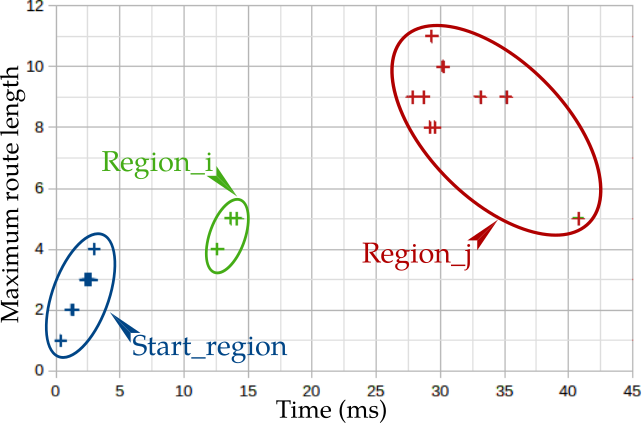
\includegraphics[scale=0.6]{figures/chapter3/performance.png}
\caption{\label{fig:chap3_performance} The resolution times of 26 places of the real mall related to the maximum route length found for each of them. The places are each on a unique and distinct path. We identify three clusters. The blue one on the left corresponds to places in the same region as the departure place. The green cluster on the center corresponds to places in a small region with few paths, different from the region of the departure place. The red cluster on the right corresponds to places in a third region with more paths in it and more interfaces to reach it. }
\end{figure}

Speaking about the division of the environment into regions, we have here circled all the measures related to places into the same region. In blue are the places being in the same region as the departure place. In green ones are places in a small region composed of 4 paths and three interfaces. In red are the places on the first floor of the building. Eleven interfaces have been identified to pass from the departure region to the first floor. The results over these three regions draw three distinct and non-overlapping clusters. Results in the same region as the departure one give resolutions under 5ms with a maximum route length of four. Results over the small region give resolutions time between 12.5ms and 15ms with routes going from 4 to 5 paths. Results over the last region create an important gap in terms of resolution time with a minimum around 28ms. 

These results could be discussed at length. On one hand, we could say that the division into regions has a positive impact on the resolution time by restricting the search space. For the places in the same region as the departure one, the paths in the other regions do not impact the search. Such an explanation would be in adequation with the presented graph. On the other hand, the ``high'' resolution times for the region in red can be attributed to this same region division. Because we want to propose several routes, and at least one passing by each interface, we artificially increase the search space with the need of at least 22 sub-routes computation for places in a region connected with 11 interfaces (one sub-route to go from the departure place to the interface and one sub-route to go from the interface to the destination place). For the smallest region (in green) 6 sub-routes computations are needed because of 3 interfaces.

To conclude the analysis of these results, we can say that regarding the need of searching several routes passing by different interfaces, the proposed algorithm is fully suitable with resolution time adapted to \acrshort{hri} applications. However, the number of interfaces linking two regions has a non-negligible impact on these resolution times. A careful description of such an environment is thus important and attention must be put on the division into regions.  

Results about the integration of the \acrshort{ssr} and its related algorithms in a robotic architecture will be provided at the end of this document over a chapter dedicated to the \acrshort{mummer} project (Chapter~\ref{chap:8}).